% !TeX spellcheck = en_GB
\documentclass[11pt]{article}
\usepackage{graphicx}
\usepackage{hyperref}
\usepackage{listings}
\title{Machine Learning Project\\Task 2}
\author{Duy Nguyen Dinh \\ dinh@rhrk.uni-kl.de\and
	Minh Duc Duong\\ duong@rhrk.uni-kl.de\and
    ---\\ ---}
\date{\today}
\begin{document}

\maketitle

\section{Data Pre-processing}

\subsection{Extract vintage from "title" column}
As the task sheet requires, we need to extract the vintage from the title column. First it is necessary to identify how would vintage appears in the title. Because they indicate a specific year, they appear mostly as a concatenation of 4 digits. The process can be done by searching for numbers using regular expression ([0-9][0-9][0-9][0-9]) in each entry of title column. This is however not enough for the exaction as there can be the case, where the 4 digits do not make any sense of year (for example: 1000 or 9000 as these should not be a reasonable years for vintage). Thus, we add some constraints with the expectation of getting more meaningful numbers for the vintage. The extracted number first should be in between 1800 and 2022 because it makes more sense that all wines were made in this year range. Also there are time when we could extracted 2 or more years in the same title entry. Here we focus on the exception with 2 different numbers. The entry 2262 in the data has 2 different years (1637 and 2002). Our implementation is to extract the maximum number as vintage, which suits this entry well because 1637 represents the establish year of the facility and 2002 is the actual wine year.

It is important to keep in mind that the extraction may not absolute accurate because the idea for the extraction of vintage comes through the observation of the data frame. For the better result, data should be consistent with a recognizable pattern.

\subsection{Histogram}
Plotting is one way to get an overview of the values of each column. There will be two types of plotting depend on the value type of columns. For numeric types (Integer or Float), we plot histograms which show the range and the distribution of values. For string type, we plot the counts of each unique values.

Because there can be too many unique values to plot, we decided to plot the counts of top 20 unique values for string columns. We also exclude description and title columns from the plot result with the assumption that each entry of these columns are unique and this makes plotting for these columns serves no purpose.

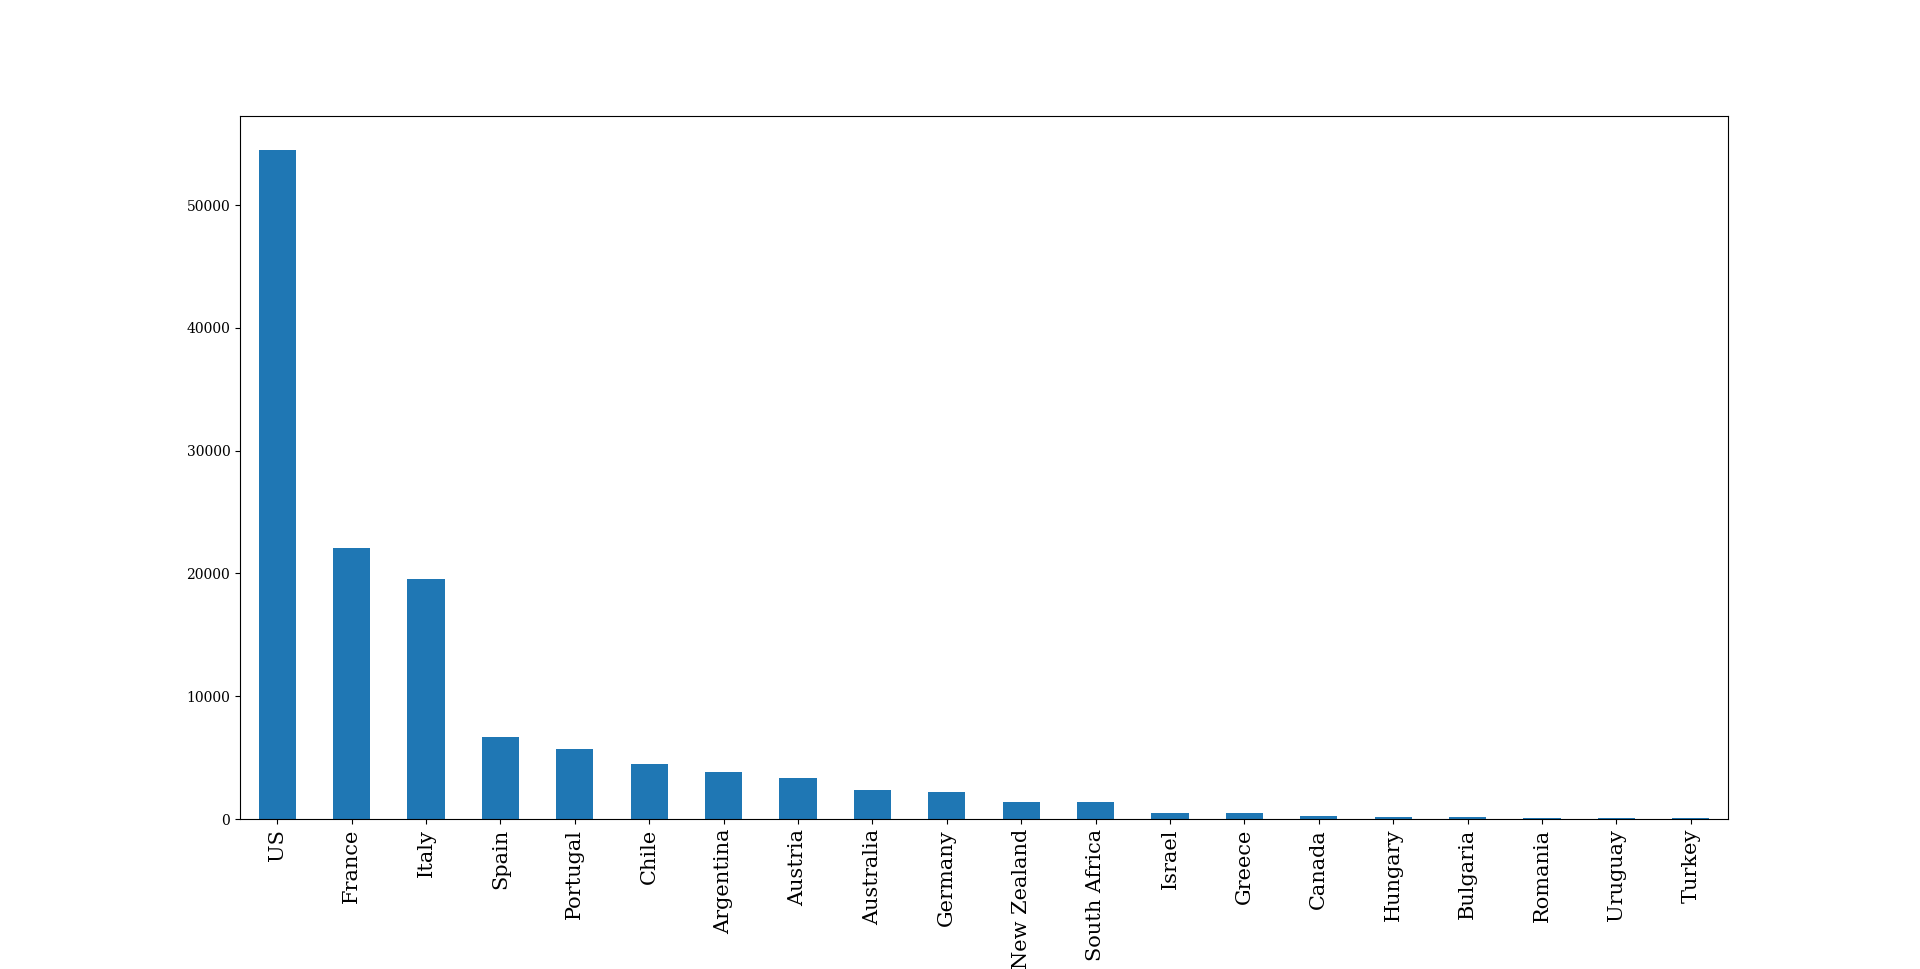
\includegraphics[width=\textwidth,height=\textheight,keepaspectratio]{figures/1c_histogram_of_country.pdf}

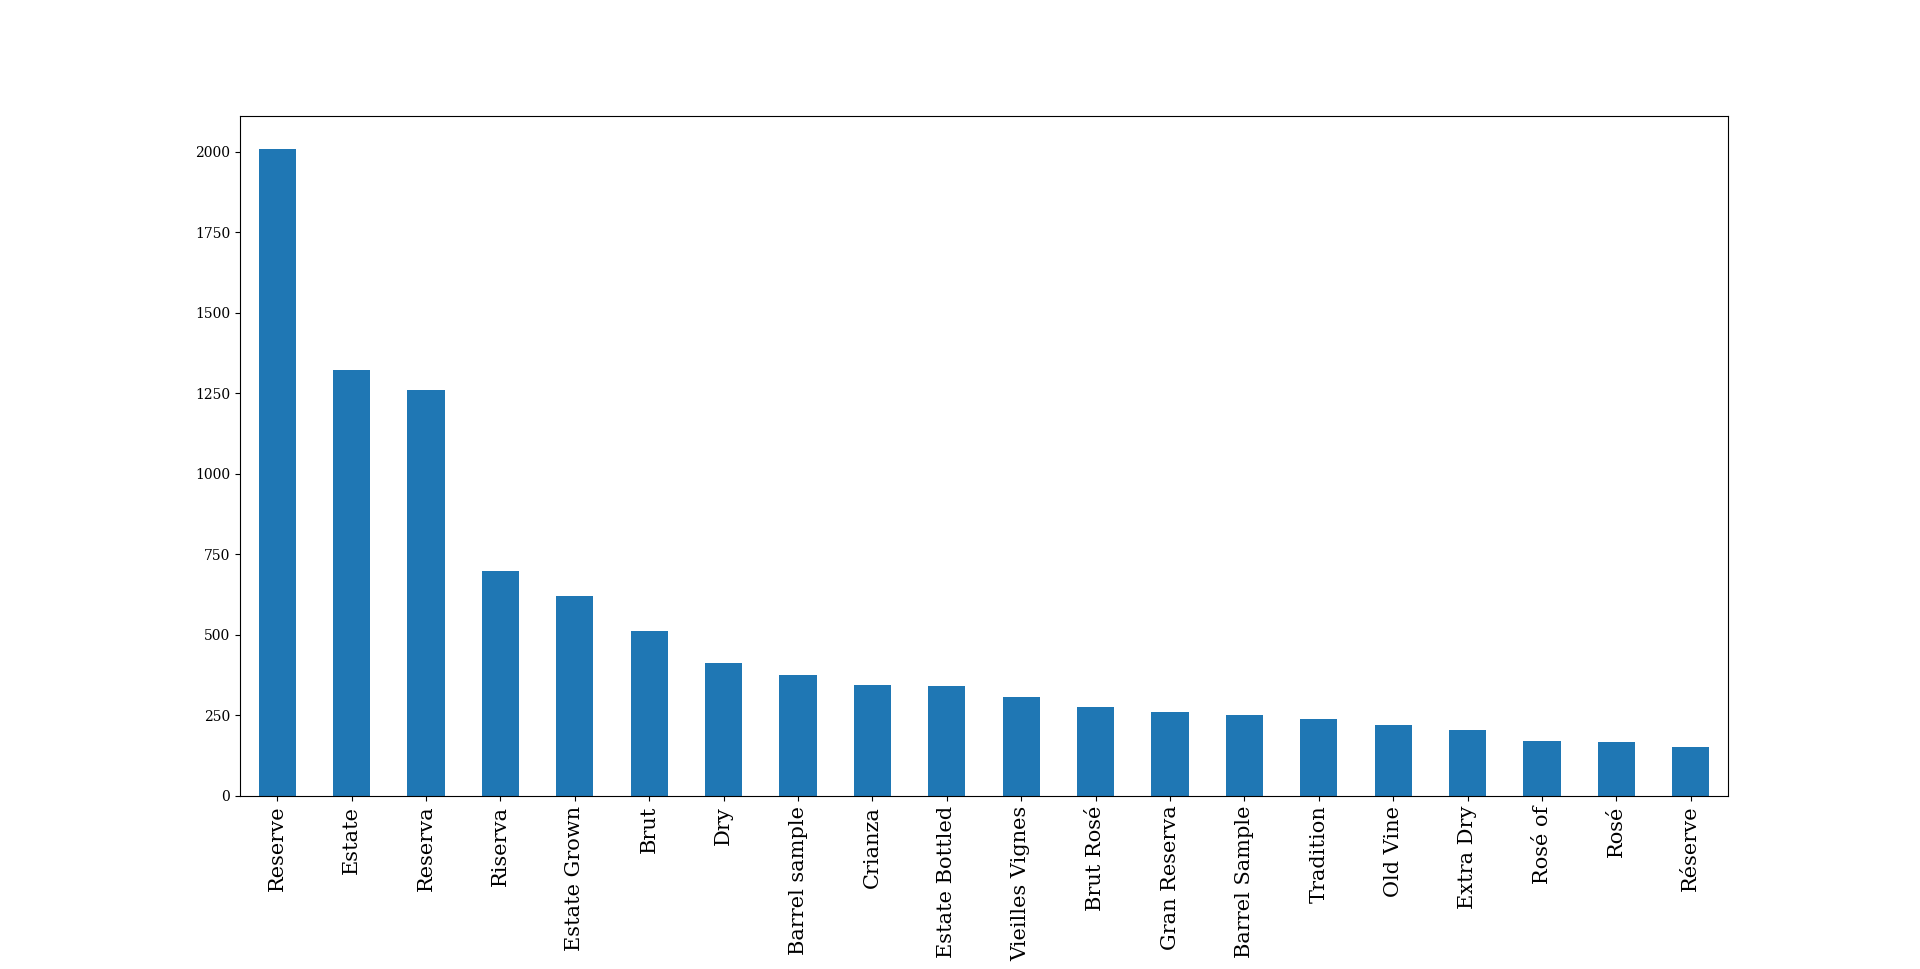
\includegraphics[width=\textwidth,height=\textheight,keepaspectratio]{figures/1c_histogram_of_designation.pdf}

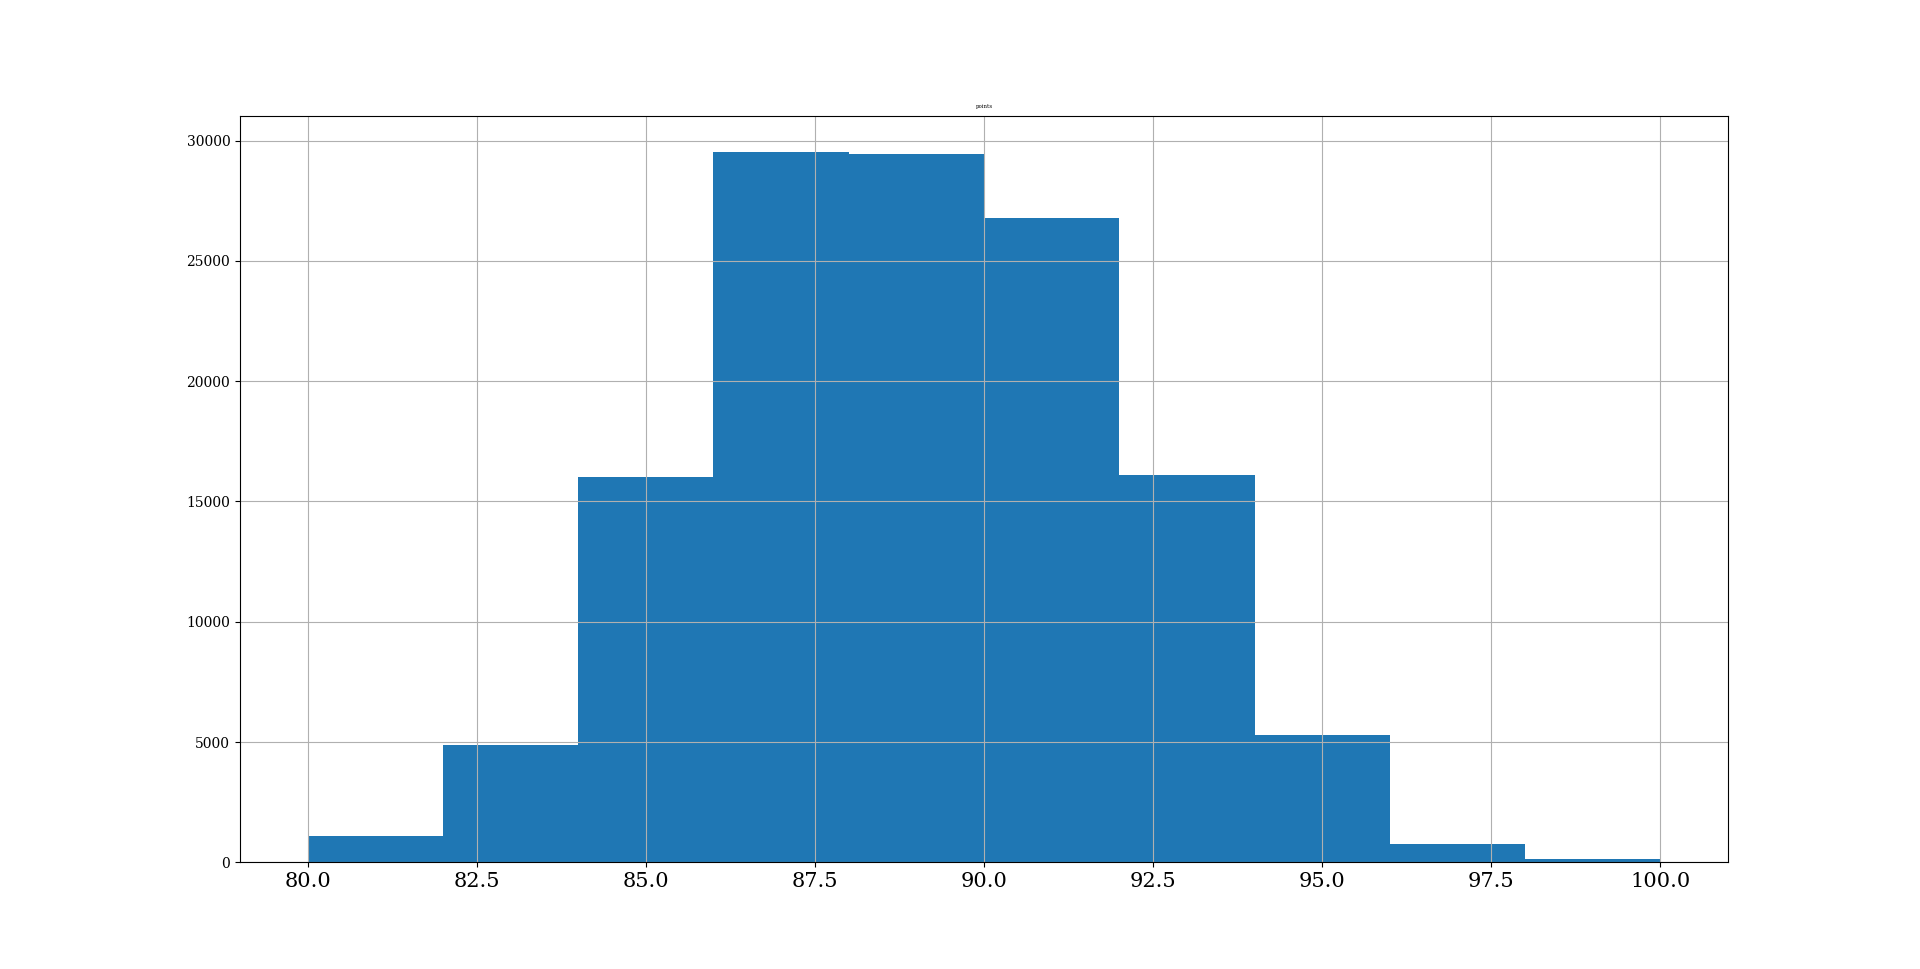
\includegraphics[width=\textwidth,height=\textheight,keepaspectratio]{figures/1c_histogram_of_points.pdf}

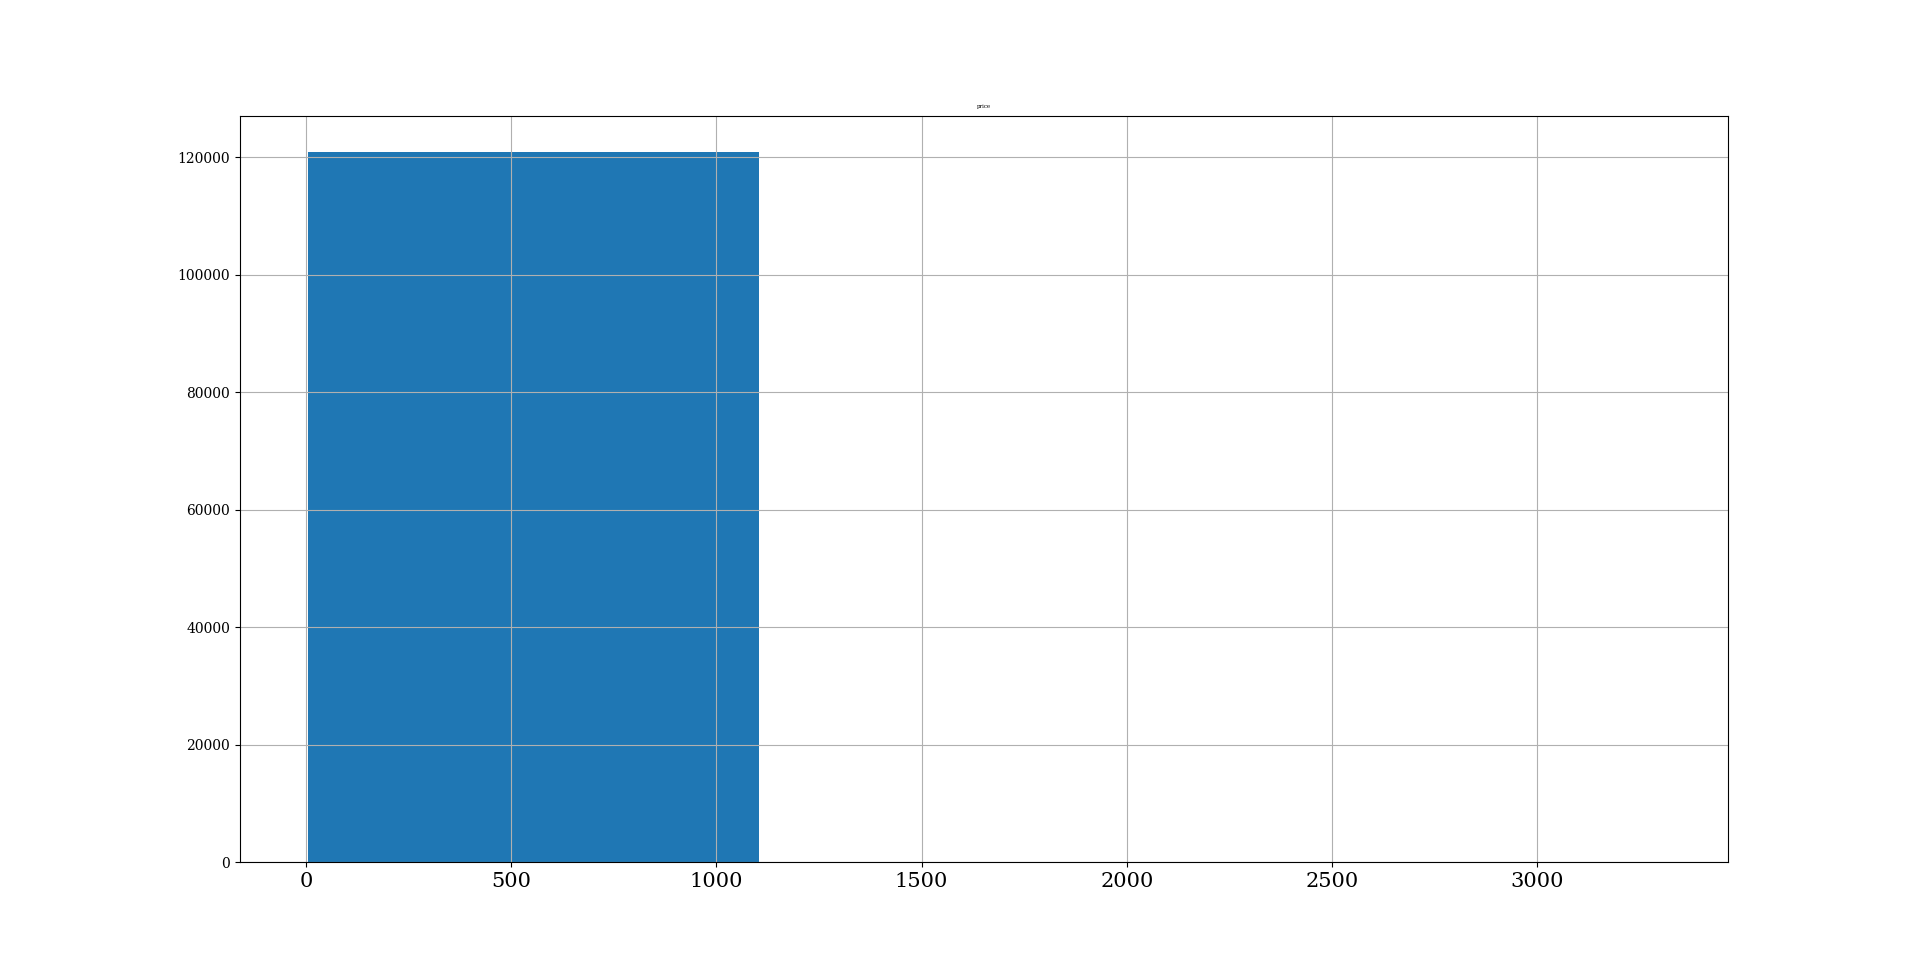
\includegraphics[width=\textwidth,height=\textheight,keepaspectratio]{figures/1c_histogram_of_price.pdf}

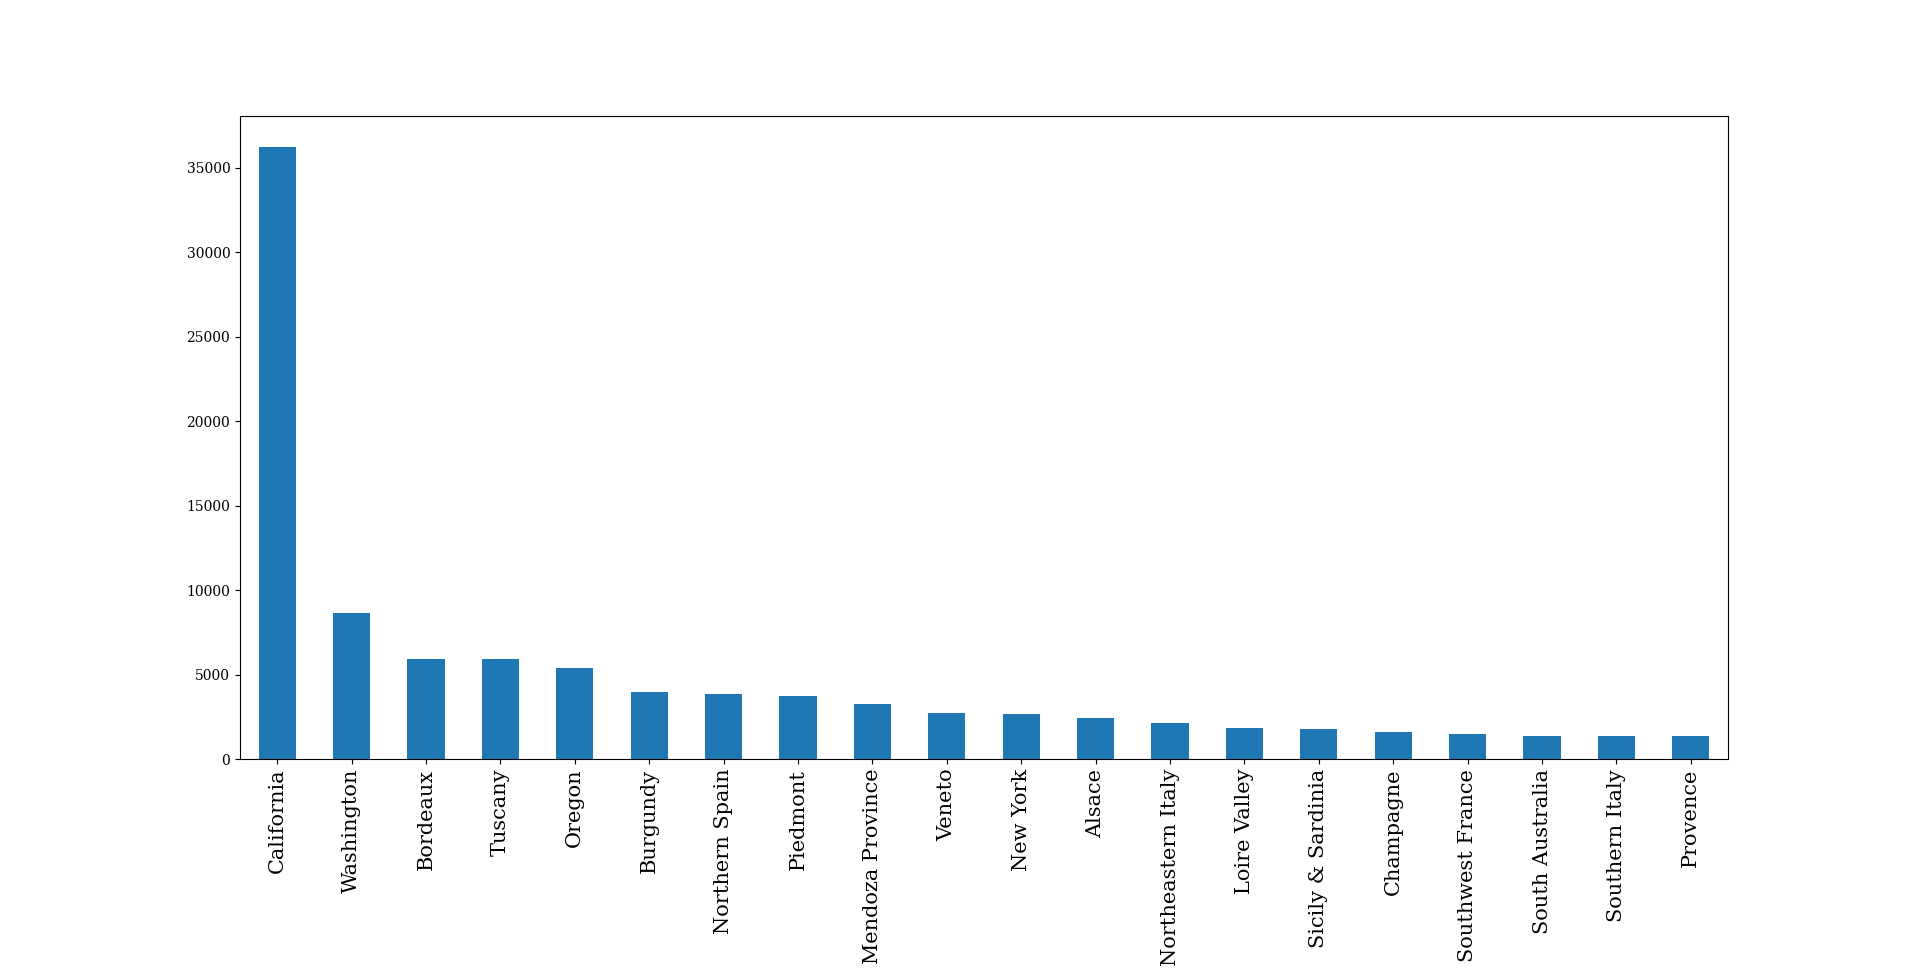
\includegraphics[width=\textwidth,height=\textheight,keepaspectratio]{figures/1c_histogram_of_province.pdf}

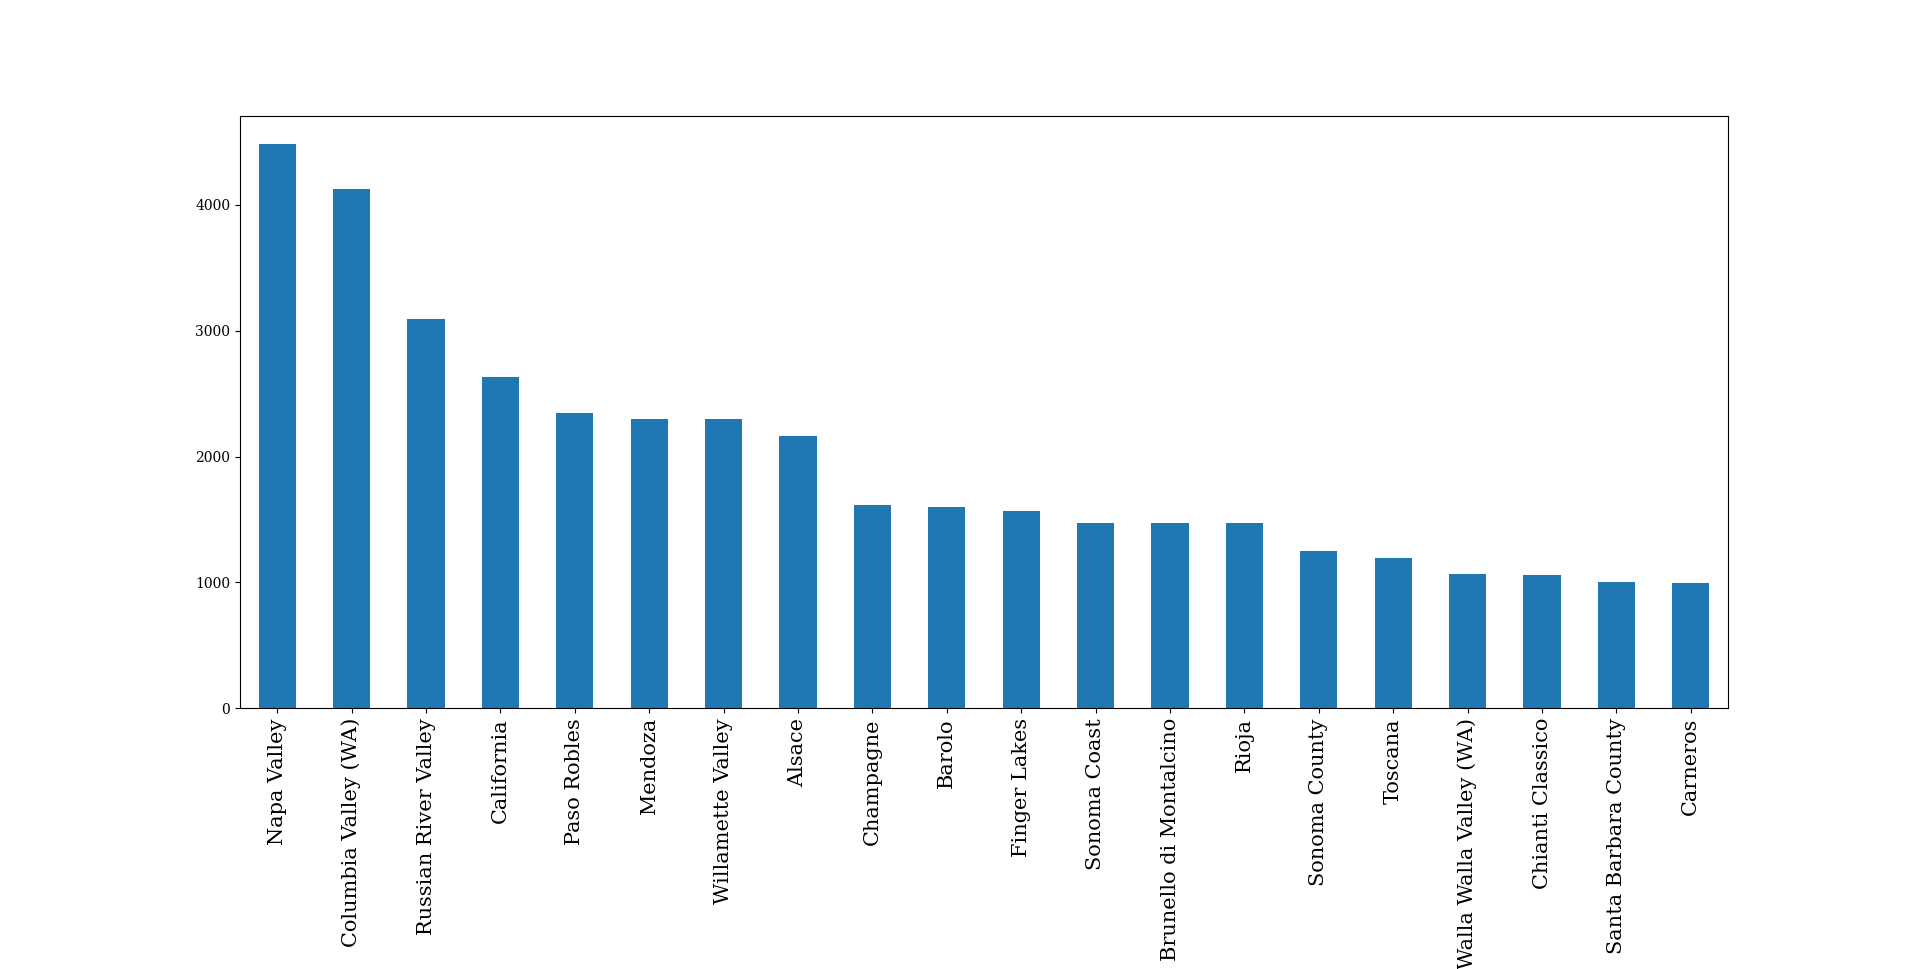
\includegraphics[width=\textwidth,height=\textheight,keepaspectratio]{figures/1c_histogram_of_region_1.pdf}

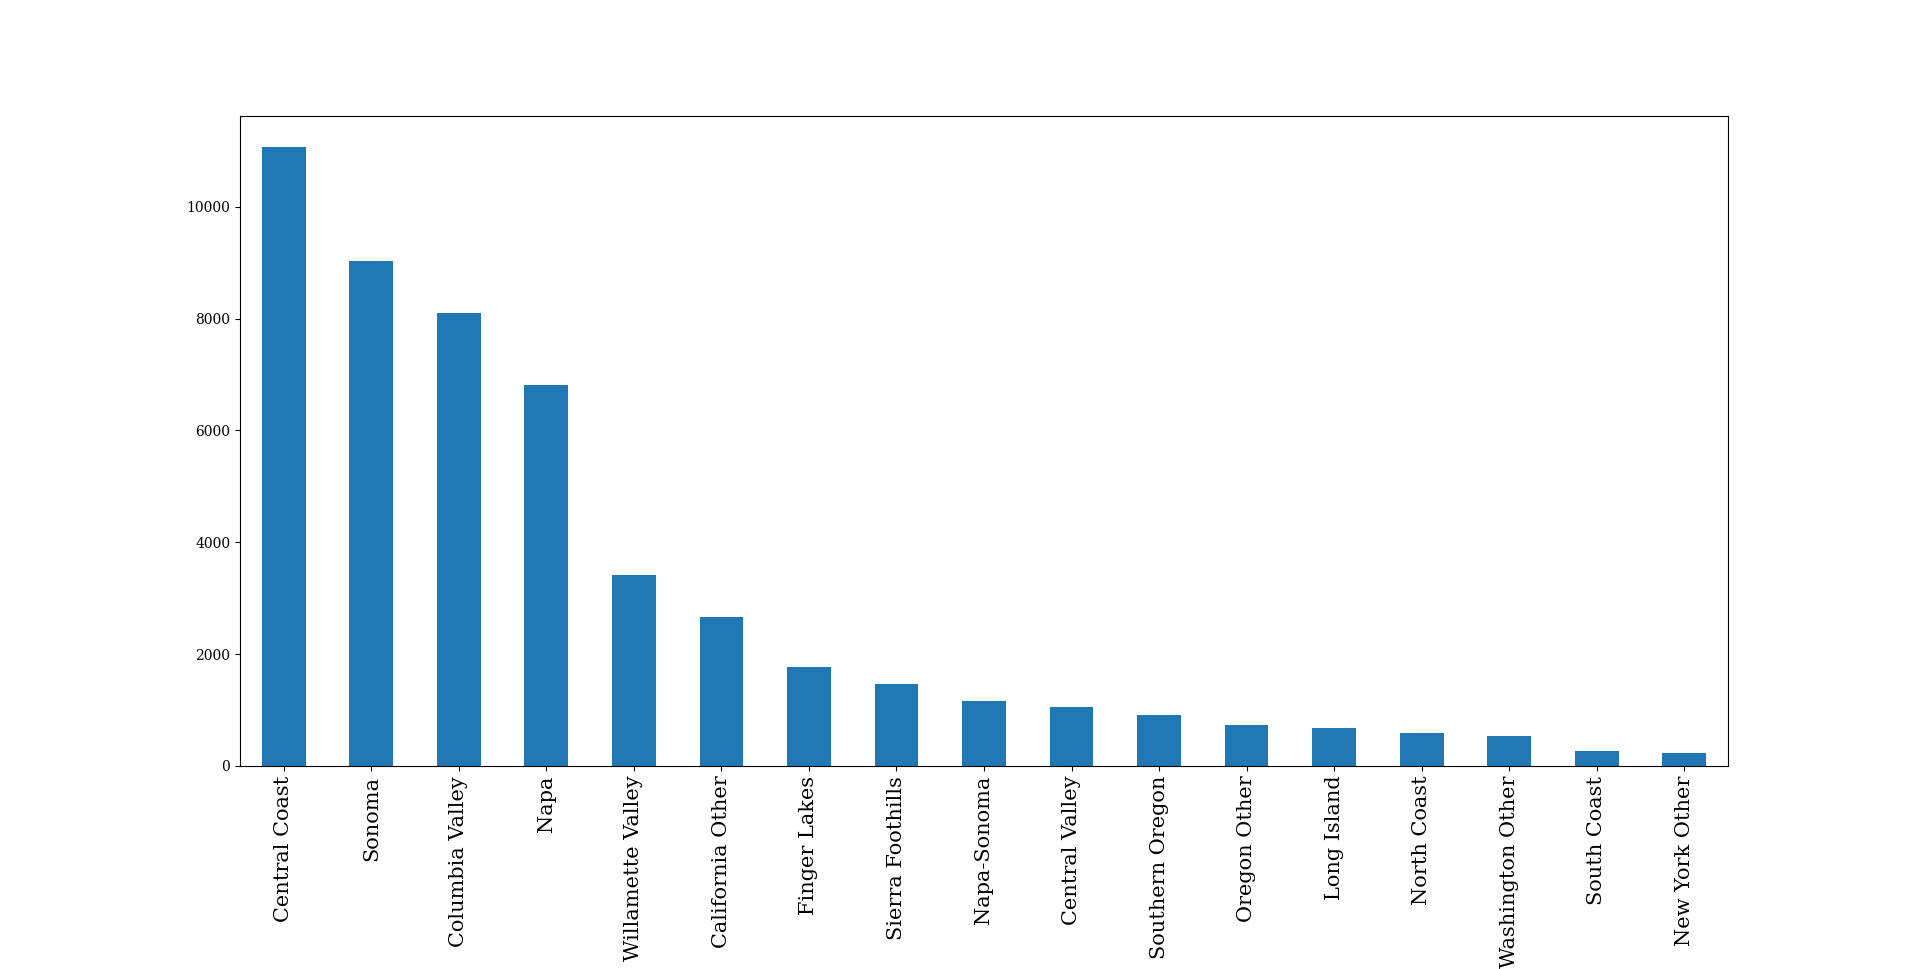
\includegraphics[width=\textwidth,height=\textheight,keepaspectratio]{figures/1c_histogram_of_region_2.pdf}

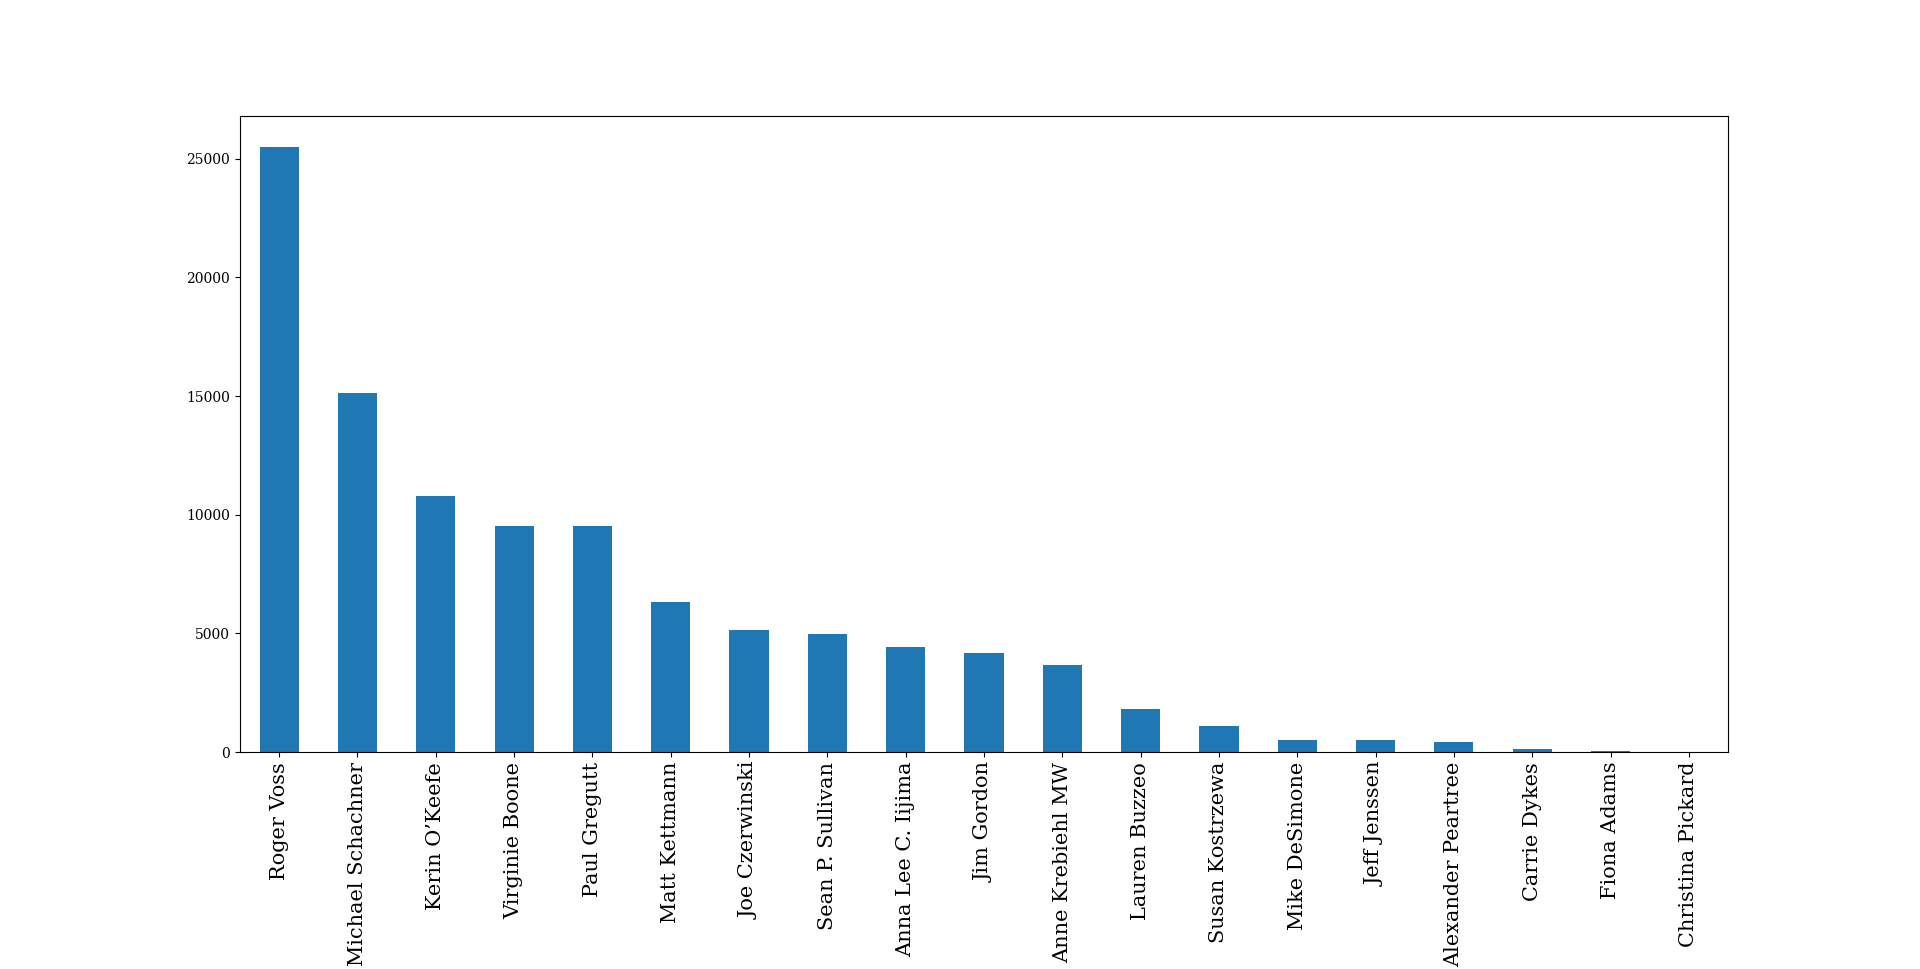
\includegraphics[width=\textwidth,height=\textheight,keepaspectratio]{figures/1c_histogram_of_taster_name.pdf}

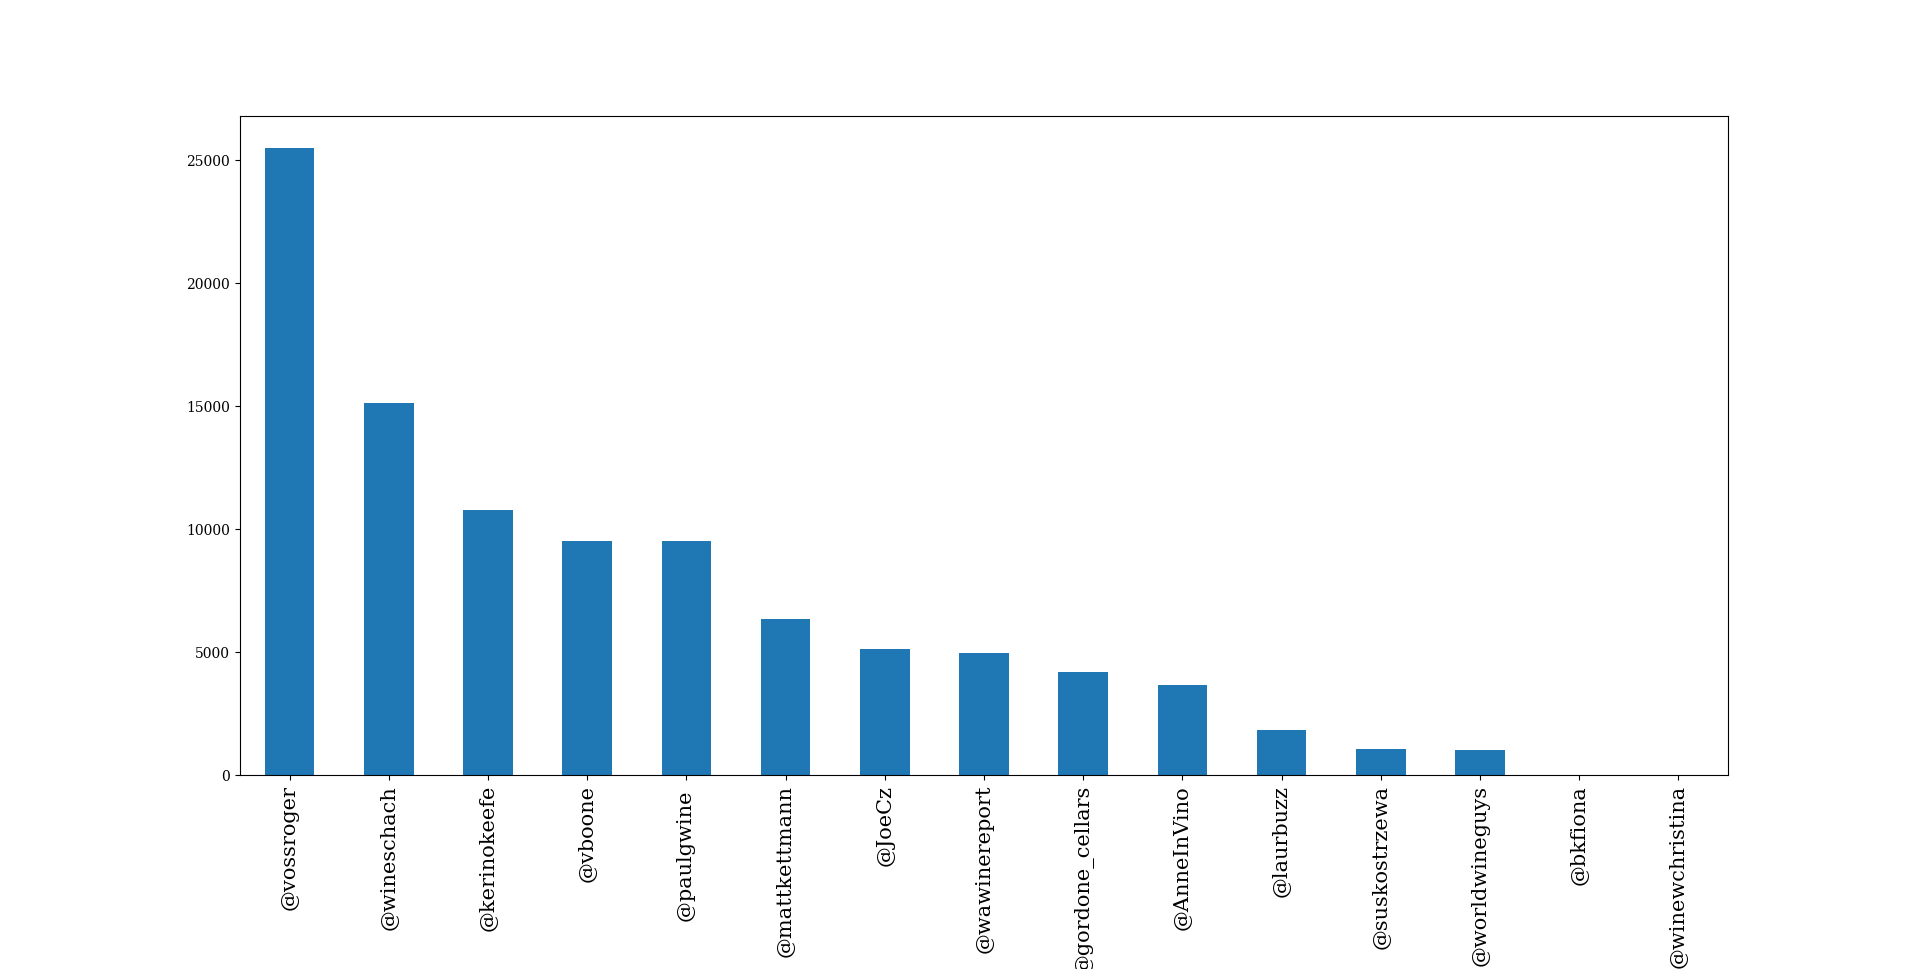
\includegraphics[width=\textwidth,height=\textheight,keepaspectratio]{figures/1c_histogram_of_taster_twitter_handle.pdf}

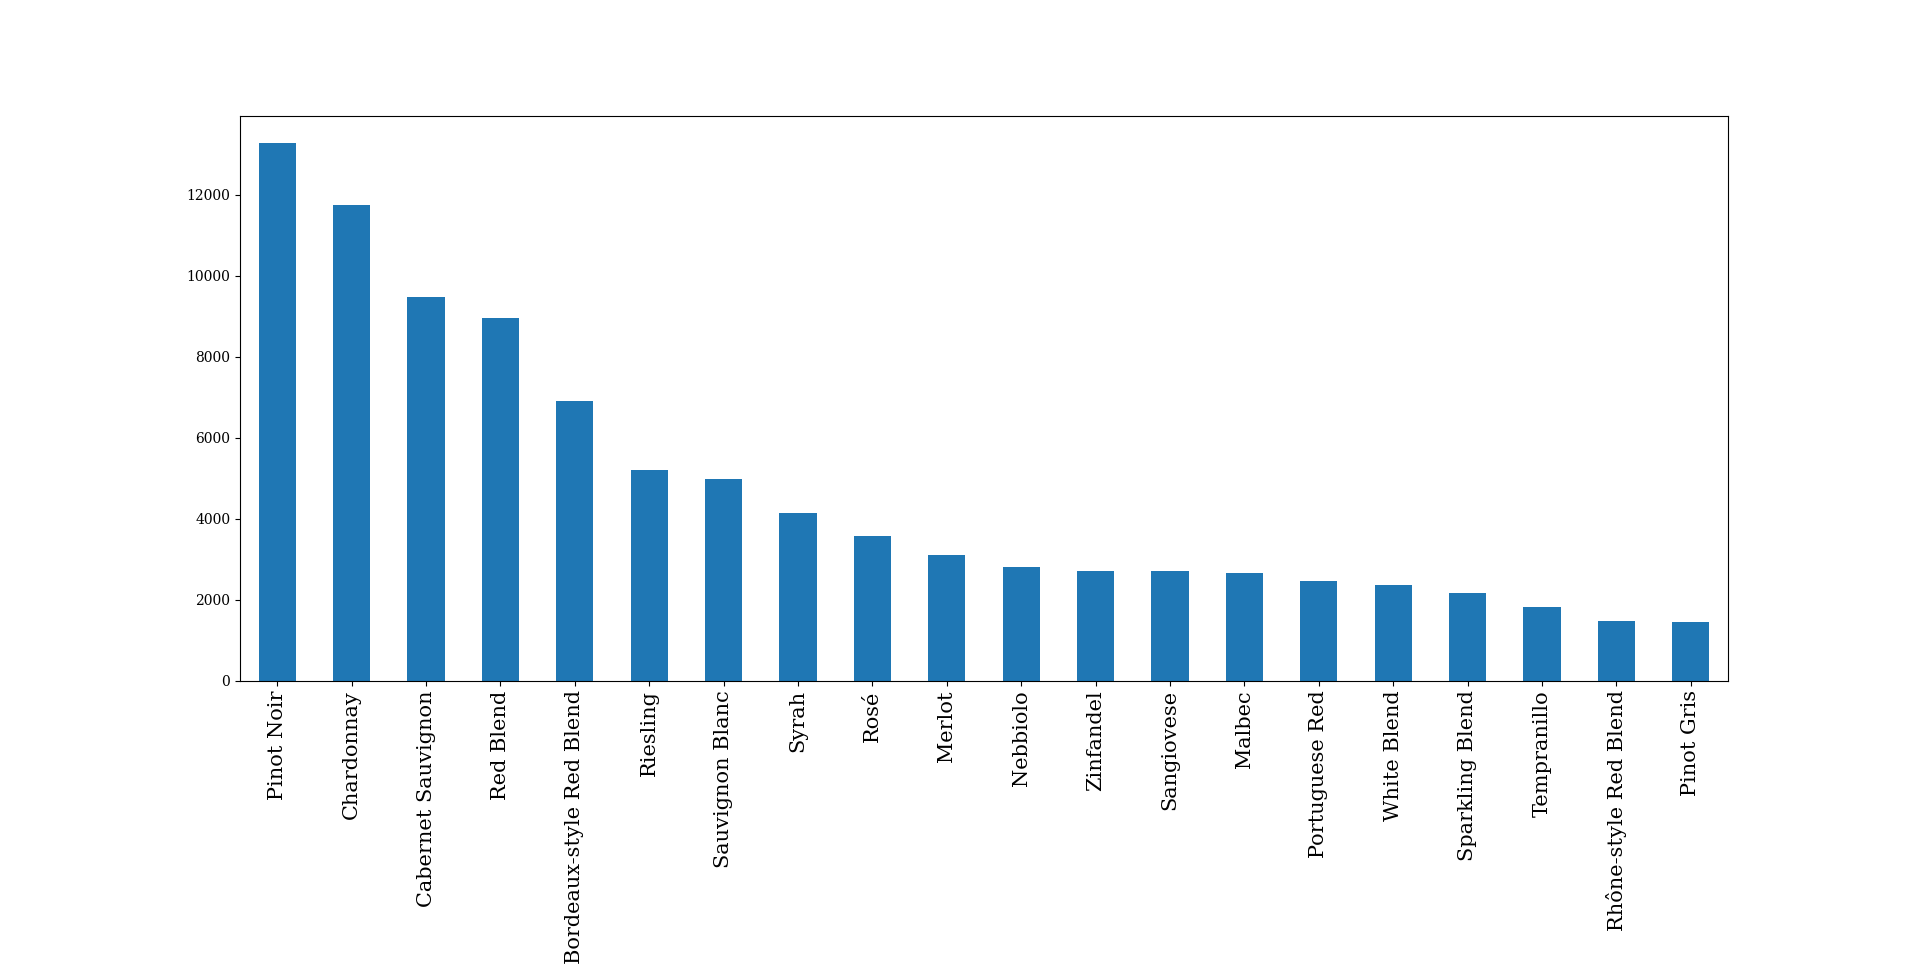
\includegraphics[width=\textwidth,height=\textheight,keepaspectratio]{figures/1c_histogram_of_variety.pdf}

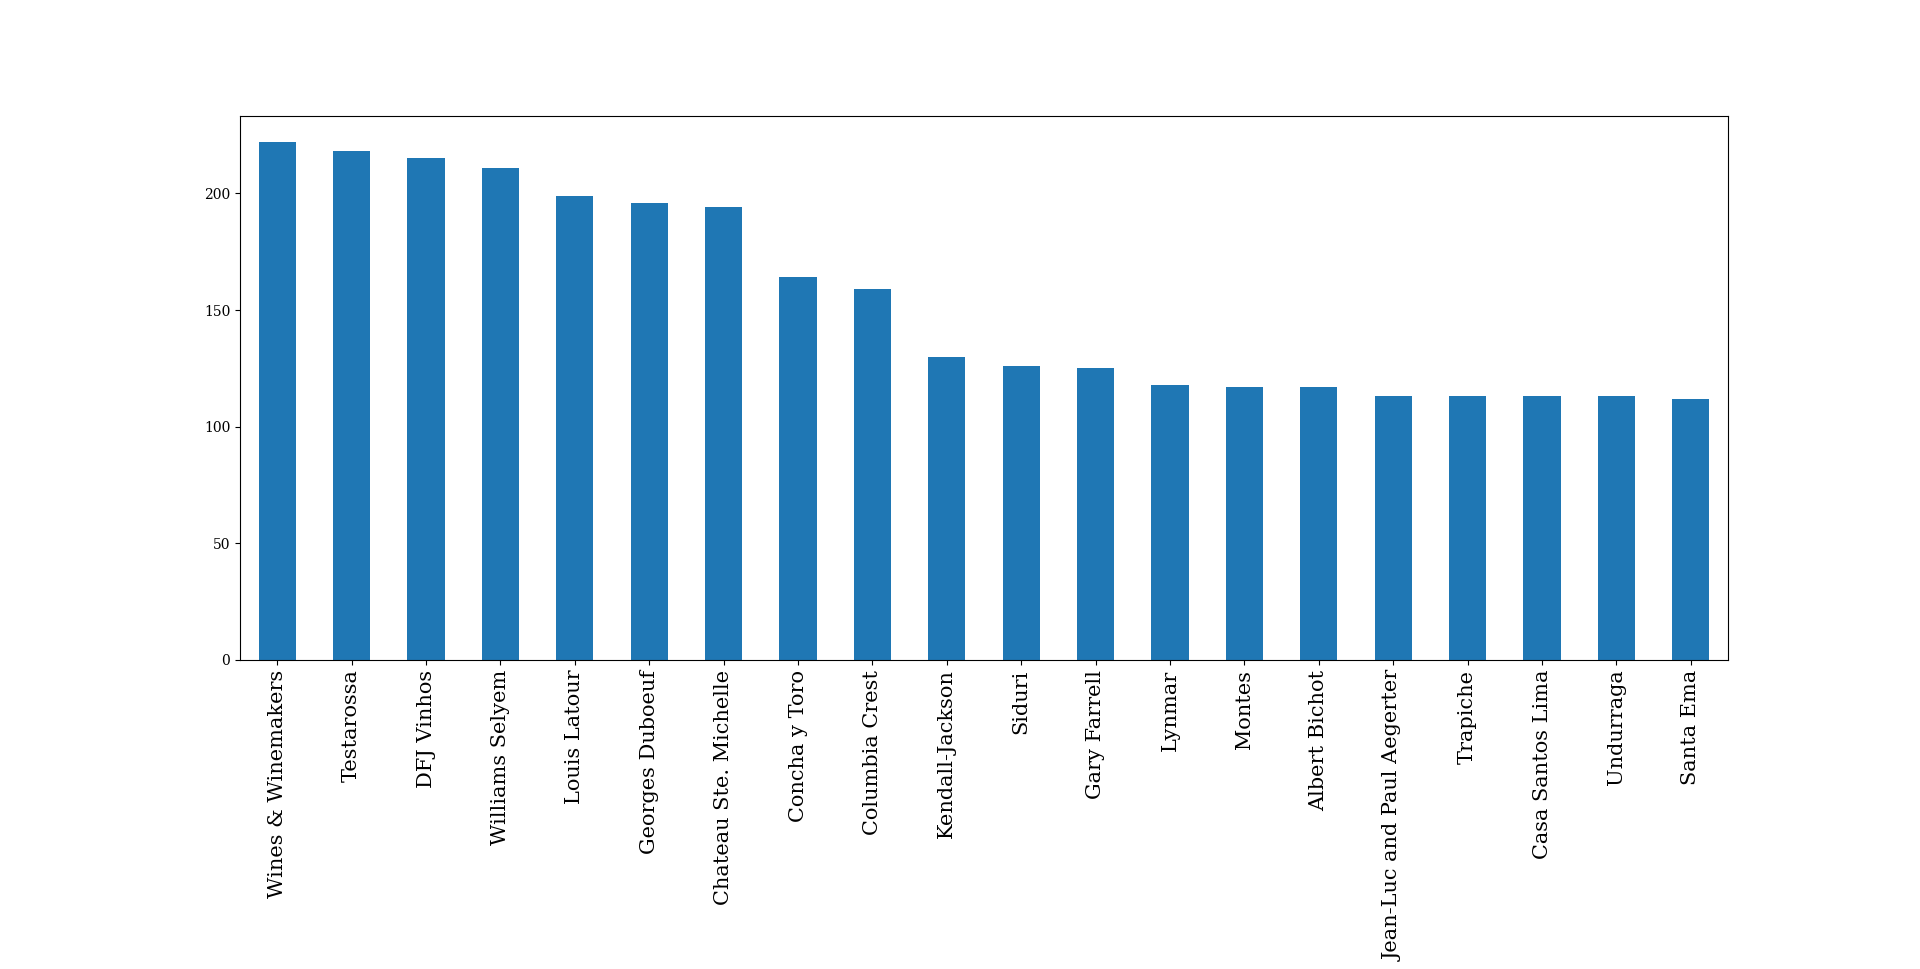
\includegraphics[width=\textwidth,height=\textheight,keepaspectratio]{figures/1c_histogram_of_winery.pdf}

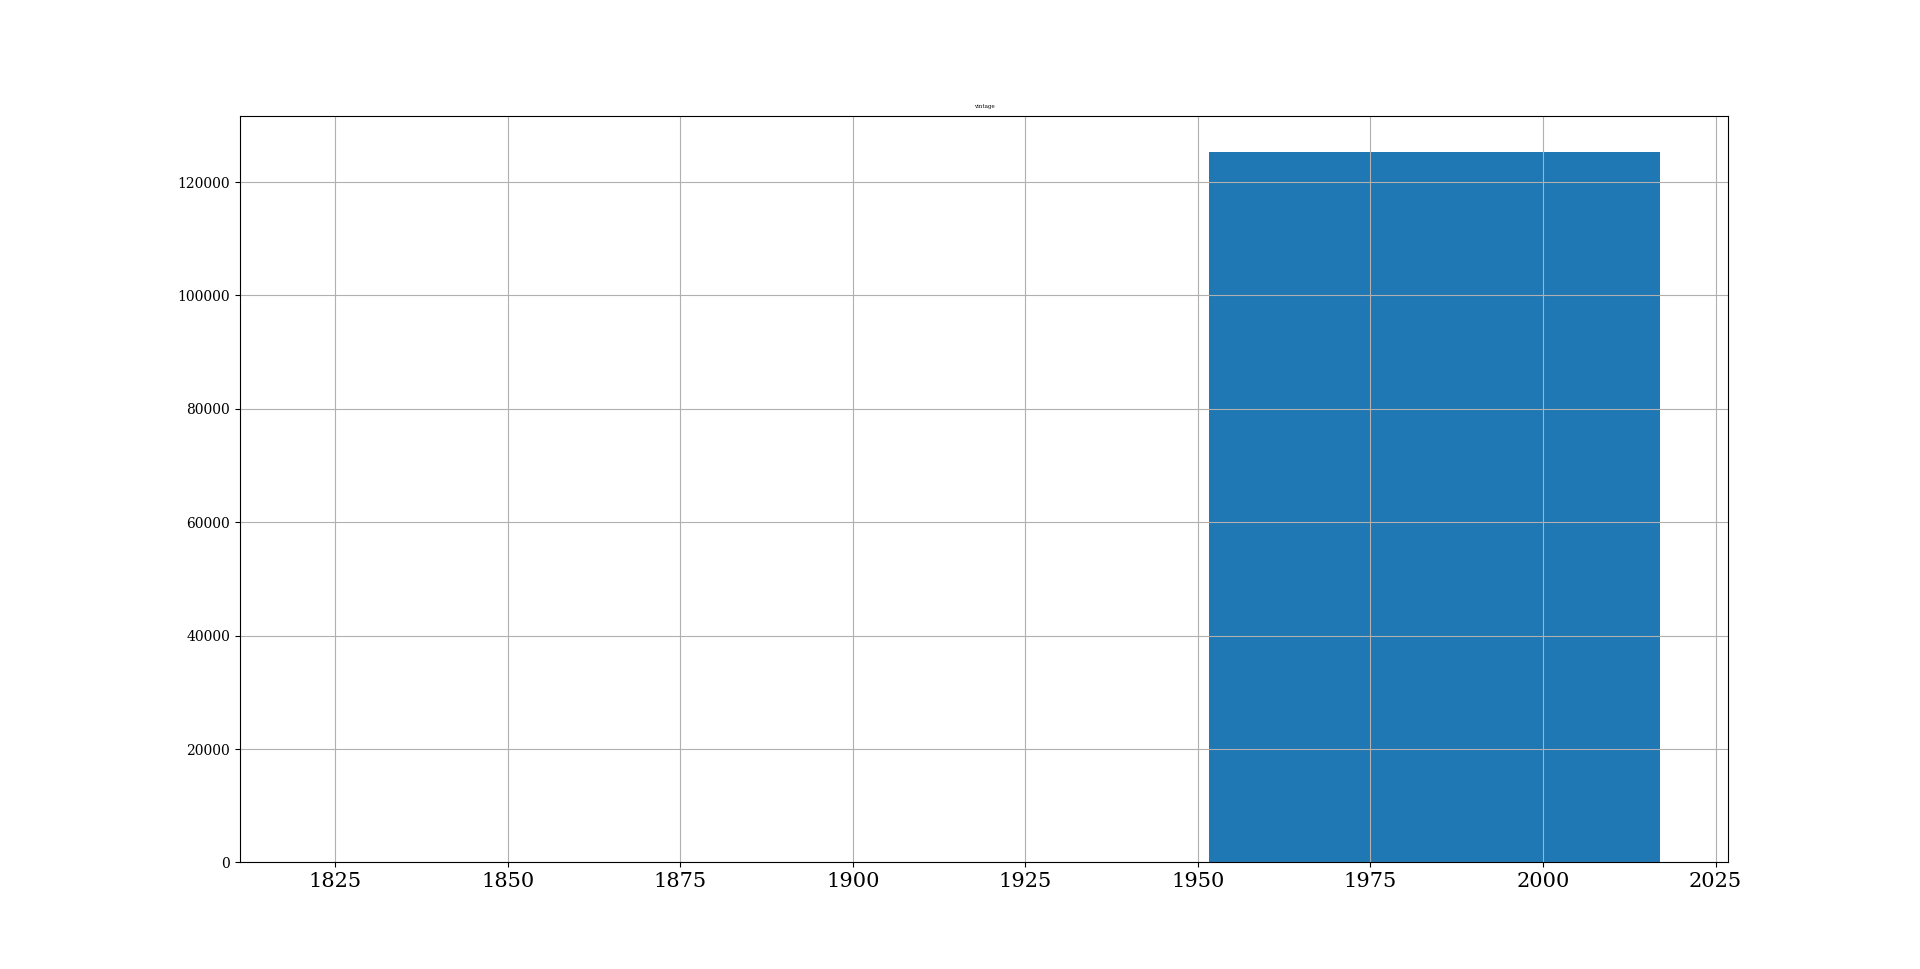
\includegraphics[width=\textwidth,height=\textheight,keepaspectratio]{figures/1c_histogram_of_vintage.pdf}

We also retrieve the number of null entries for each column:

\begin{itemize}
    \item country                     63
    \item description                  0
    \item designation              37465
    \item points                       0
    \item price                     8996
    \item province                    63
    \item region\_1                 21247
    \item region\_2                 79460
    \item taster\_name              26244
    \item taster\_twitter\_handle    31213
    \item title                        0
    \item variety                      1
    \item winery                       0
    \item vintage                   4611
\end{itemize}

\subsection{Statistics}

We calculate 5 insights for the numerical data: minimum, maximum, mean, median, standard derivation. Because the data is standardized in the pre-processing phase, the means are nearly 0, the standard derivations nearly 1.

\begin{lstlisting}
BEGIN COMPUTING STATS
.
price_minimum = -0.792466772305429
price_maximum = 82.48840796649863
price_mean = 0.0005821718408075238
price_median = -0.18605263585782666
price_std = 1.0006138616970786
.............................
.
vintage_minimum = -1.5879808275786031
vintage_maximum = 47.52570036289124
vintage_mean = -0.0013231589048437516
vintage_median = -0.08450079113564869
vintage_std = 0.9975200577812415
.............................
END COMPUTING STATS
\end{lstlisting}

\subsection{Data Transformation}

In this task, we transform each column individually and force each output to be a 2d matrix and have the same shape at the second dimension, so that after the transformation we can concatinate all the results to fit the model.\\

For categorical data, we set the rare values to 'Other'. For example, If the there is 2 records come from Egypt and the \textbf{min\_count} equals 3, then the country is set to 'Other'.
\begin{lstlisting}[language=python]
content.mask(content.map(content.value_counts()) < min_count, 'Other')
\end{lstlisting}

We set the threshold of missing data on each row to 2. It means for example, a row that misses the country and province will be removed from the dataset. 
\begin{lstlisting}[language=python]
data.dropna(thresh=data.shape[1]-3)
\end{lstlisting}

Data from the columns will be classified into 3 types: numerical, categorical and text data:

Numerical data includes \textbf{price}, \textbf{vintage}, \textbf{points}. For this data type, we reshape it from an 1d-array to a (N,1) matrix. Missing data will be fulfilled with the mean of the presenting data. We observe their standard deviation to assess the impact on the related weight of the model. When the impact if an column is huge, we standardize it with \textbf{StandardScaler} \footnote{\url{https://scikit-learn.org/stable/modules/generated/sklearn.preprocessing.StandardScaler.html}}.

Only the \textbf{description} column includes text data. First, texts will be tokenized and stop words and other with frequency less than 2 will be filtered out. Then a dictionary is created by the remaining words. We use \textbf{Doc2Vec} model\footnote{\url{https://radimrehurek.com/gensim/models/doc2vec.html}} to vectorize the description string. Next, the model will be trained for 20 \textbf{epochs}. Finally, the model transform each description into a vector with \textbf{vector size} 50.

The rest are categorical data. We can see also a set of hierachical type: \textbf{country}, \textbf{province}, \textbf{region\_1}, \textbf{region\_2}. There are plenty of encoding technics for that type of data. In this project we use mainly three methods: Sum encoding, Binary encoding, Target encoding. Sum encoding will be applied to the columns with a small set of categories like \textbf{taste\_name}, \textbf{province}. It is an efficient method which represent the nature of categorical variable's encoding, but memory and runtime are the trade-off. In Sum encoding, missing data will be set to a vector of minus one. For columns that have a huge amount of categories and a small impact on the target column, we use binary encoding to reduce the features. The involved columns include \textbf{region\_1} (1229 categories to 11 binary features), \textbf{variety} (707 to 10). We apply target encoding on \textbf{country}, \textbf{designation}, \textbf{winery}. Target encoding would lead to overfitting, therefore we use the version with additive smoothing. In this encoding, missing data will be set to the general mean.

We realized that \textbf{taster\_twitter\_handle} data is identical with taster\_name, when it exists. So, we decide to transform it into a boolean feature, expresses that whether the taster has a taster account. the tranformed data has only one variable, the feature correlation between \textbf{taster\_name} and \textbf{taster\_twitter\_handle} is eliminated.

\textbf{title} is just the concatination of designation, vintage, variety, winery. Therefore, we ignore this column.

\subsection{New data prediction after pre-processing train data}

For categorical data: When a new category is detected, we still need some constraints to check if this is actual new. For example, with a specific implementation, "US", "USA" and "America" in column country are totally different. This means we need a way to pre-process the values for each categorical column and different input values with the same context should be grouped together. Next, when we have actually a new category from new data, it is problematic, since we use one-hot encoding for certain columns, which leads to missmatch of vector dimension size. Also in the case of standardized numerical data, new incoming data will make a huge change of the mean and derivation. Therefore, the solution is to merge the train data with the test data, then pre-process them together.

For Doc2Vec model: When we reach a specific number of newly added rows, the Doc2Vec model for description column should be trained again with the new incoming data to enrich the vocabulary.
\section{Ridge Regression}

\subsection{Ridge Regression with Bias}

The Ridge Regression with Bias is built on top of the one without bias. We extend each record of entry dataset by a constant (with numpy method \textbf{np.c\_}), which represents for the bias.

\begin{lstlisting}[language=python, caption=KNN class]
    class RidgeRegressionBias:
    def __init__(self, C=1):
        self.rr = RidgeRegression(C)

    def fit(self, X, y):
        data_size = len(y)
        X = np.c_[X, np.ones(data_size)]
        self.rr.fit(X,y)

    def predict(self, X):
        data_size = len(X)
        X = np.c_[X, np.ones(data_size)]
        return self.rr.predict(X)
\end{lstlisting}

\subsection{Relationship of ``points" column with other}

In the plots below, we draw the linear functions of Ridge Regression (with Bias) model right on the scatter plot of the fitted data points. Therefore, we can see the derivation of the data points from the function.

Some plot like \textbf{country} and \textbf{taster\_name}, we use one-hot encoding and PCA projection to reduce the number of dimensions to 1. Therefore, the distribution of data points is clustered.

\textbf{designation} and \textbf{winery} in the another hand are target encoded. The distribution of data points has the shape of a parallelogram. the quality of this encoding can be measured by the standard derivation of encoded data (the smaller the better). Therefore, the vertical width of the parallelogram should be small.

\includegraphics[width=\textwidth,height=\textheight,keepaspectratio]{figures/2b_country.pdf}
\includegraphics[width=\textwidth,height=\textheight,keepaspectratio]{figures/2b_description.pdf}
\includegraphics[width=\textwidth,height=\textheight,keepaspectratio]{figures/2b_designation.pdf}
\includegraphics[width=\textwidth,height=\textheight,keepaspectratio]{figures/2b_price.pdf}
\includegraphics[width=\textwidth,height=\textheight,keepaspectratio]{figures/2b_province.pdf}
\includegraphics[width=\textwidth,height=\textheight,keepaspectratio]{figures/2b_region_1.pdf}
\includegraphics[width=\textwidth,height=\textheight,keepaspectratio]{figures/2b_region_2.pdf}
\includegraphics[width=\textwidth,height=\textheight,keepaspectratio]{figures/2b_taster_name.pdf}
\includegraphics[width=\textwidth,height=\textheight,keepaspectratio]{figures/2b_vintage.pdf}
\includegraphics[width=\textwidth,height=\textheight,keepaspectratio]{figures/2b_variety.pdf}
\includegraphics[width=\textwidth,height=\textheight,keepaspectratio]{figures/2b_winery.pdf}


\subsection{Forward step selection}
We want to find the most impact features in the data and forward step selection is one of the options. We first start with an empty model with no fitted data, then we find the best feature to add to the model. This can be done base on the mean squared errors when we add each available feature to the model. We keep adding features into the model until we reach a certain number k.

As for the result of the given wine data:
\begin{itemize}
    \item k=0: Feature: description with the mse of 596.297918013402
    \item k=1: Feature: country with the mse of 5.609319585427947
    \item k=3: Feature: province with the mse of 4.878210024539221
    \item k=4: Feature: taster\_name with the mse of 4.75865561866921
\end{itemize}

The most significant features are the one with many unique values across the data (description, country) because the column with more unique values will contain better relations with other column. On the other hand, if most row cluster into a certain value or range of values (price/points/vintage), this makes prediction harder because the values do not hold any meaning for a good estimation (as completely different wine can have the same points).

% Print references
\end{document}
